\documentclass[11pt]{beamer}
\usepackage{amsmath}
\usepackage{graphicx}
\usepackage{tikz}
\usepackage{array}
\usepackage{pgflibraryshapes}
\usepackage[utf8]{inputenc} 
\usepackage[francais]{babel} 

\makeatletter
\begin{document}

\title[Attaques timings contre les caches des CPU]{\textit{Attaques timings contre les caches des CPU} }

\author[Jean BAUDINAT, Chloé MACUR]{Jean BAUDINAT, Chloé MACUR}

\institute[Télécom ParisTech]
{\scriptsize{Télécom ParisTech\\ \vspace{0.2cm} 
  }
}
\date[\thedate]{\footnotesize{\textsl{SSE} - 22 Juin 2015}}

\begin{frame}
  \titlepage
\end{frame}

\section*{Plan}
\addtocounter{section}{-1}
\begin{frame}{Plan} 
  \tableofcontents%[hideallsubsections]
\end{frame}

%\AtBeginSection[]
%{
%  \begin{frame}<beamer>
%    \frametitle{Plan}
%    \tableofcontents[currentsection,subsection]
%  \end{frame}
%}



\section[Fonctionnement du cache]{Fonctionnement du cache}

\begin{frame}{Fonctionnement du cache}
TODO
\begin{figure}[h]
  \centering
  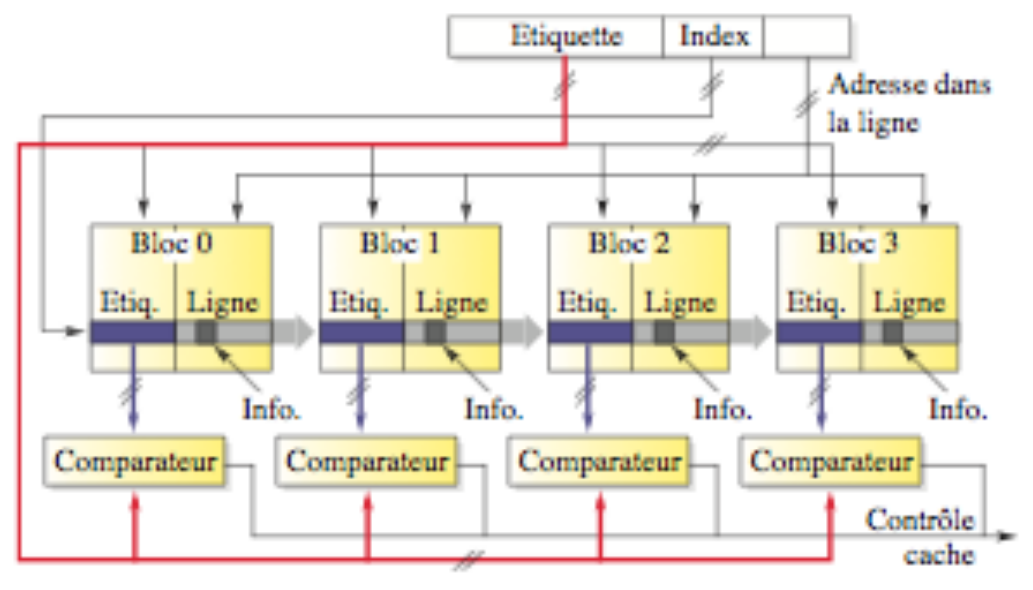
\includegraphics[width=7.5cm]{figures/cache_associative.png}
  \caption{Caches associatifs par blocs (\emph{4-way set associative})}
  \label{cache} 
\end{figure}
\end{frame}

\section{Fonctionnement de l'attaque : l'exemple d'AES}

\subsection{Vulnérabilité d'AES}
\begin{frame}{Vulnérabilité d'AES}
TODO \emph{Cache Timing Attack} 
\end{frame}

\subsection{Types d'attaques}
\begin{frame}{Types d'attaques}
TODO \emph{Cache Timing Attack} 
\end{frame}

\section{Mise en place concrète de l'attaque}

\subsection{État initial du cache} 
\begin{frame}{État initial du cache}
TODO \emph{Cache Timing Attack} 
\end{frame}

\subsection{Attaques synchrones et asynchrones}
\begin{frame}{Attaques synchrones et asynchrones}
TODO \emph{Cache Timing Attack} 
\end{frame}

\subsection{Mesure du temps}
\begin{frame}{Mesure du temps}
TODO \emph{Cache Timing Attack} 
\end{frame}

\section{Contre-mesures}

\subsection{Une attaque sur x86 plus difficile}
\begin{frame}{Une attaque sur x86 plus difficile}
TODO \emph{Cache Timing Attack} 
\end{frame}

\subsection{Une évolution des technologies créatrice de difficultés supplémentaires}
\begin{frame}{Une évolution des technologies créatrice de difficultés supplémentaires}
TODO \emph{Cache Timing Attack} 
\begin{figure}[h]
  \centering
  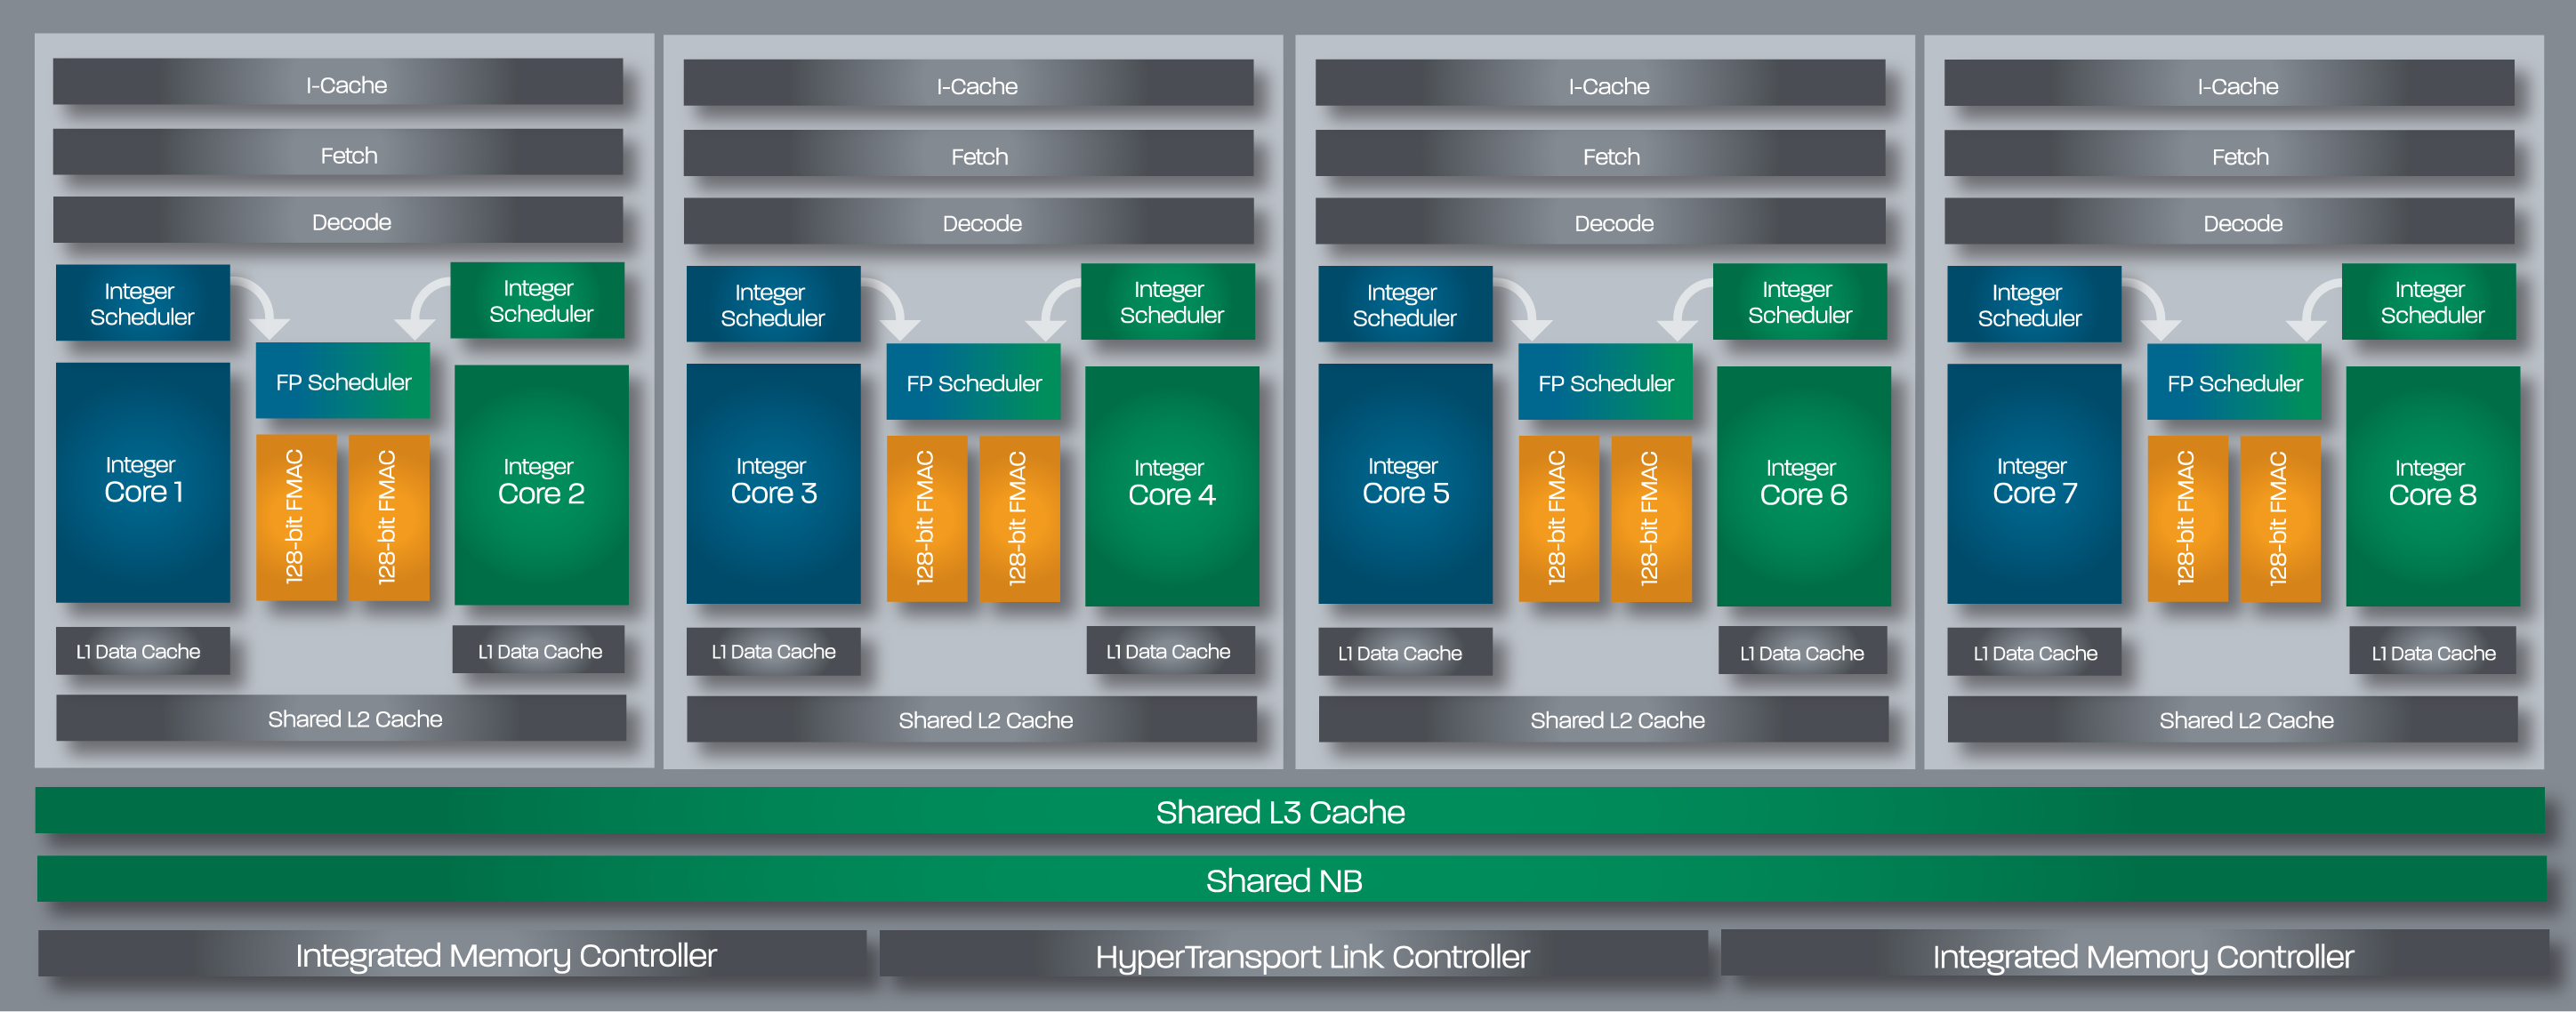
\includegraphics[width=8cm]{figures/BDArch.png}
  \caption{Étagement des caches dans un processeur quadricoeur}
  \label{etagement} 
\end{figure}
\end{frame}

\subsection{Implémentation d'un algorithme en temps constant: le cas d'AES}
\begin{frame}{Implémentation d'un algorithme en temps constant: le cas d'AES}
TODO \emph{Cache Timing Attack} essai~\cite{canteaut2006understanding}
\end{frame}

\section*{Conclusion et  références}
\frame[allowframebreaks]{

\begin{block}<+->{Perspectives}
lala. 
\alert{conclu} bla
\end{block}
\vspace{1cm}
\bibliographystyle{plain}
{\tiny \bibliography{ref}}
}

\end{document}
